% Non-official two-column ICML-like draft. See README before submission.
% Every numerical table is generated from saved predictions by analyze_results.py.
\documentclass[10pt,twocolumn,letterpaper]{article}
\usepackage[margin=0.75in,columnsep=0.25in]{geometry}
\usepackage[T1]{fontenc}
\usepackage{lmodern}
\usepackage{amsmath,amssymb,booktabs,graphicx,tabularx,microtype}
\usepackage[round,authoryear]{natbib}
\usepackage[hidelinks]{hyperref}
\usepackage{caption}
\captionsetup{font=small,labelfont=bf}
\setlength{\parindent}{1em}
\setlength{\parskip}{0pt}
\title{Class Weighting at a Fixed Decision Threshold:\\A Burst-Level Case Study in Hydraulic Pump Condition Monitoring}
\author{Anonymous draft}
\date{}
\begin{document}
\maketitle

\begin{abstract}
Inverse-frequency class weighting is a reasonable response to rare positive labels, but its effect depends on representation and decision threshold. We examine a saved logistic-regression experiment on 575 normal and 20 abnormal vibration bursts using five fixed summary features and identical five-fold cross-validation repeated ten times. At probability threshold 0.5, unweighted and balanced models detect the same 18 abnormal bursts in all ten appearances and miss the same two. Balanced weighting adds 94 false-positive out-of-fold observations from 16 normal bursts, reducing mean fold F1 from 0.942 to 0.776 while increasing ROC-AUC from 0.917 to 0.948. Trapezoidal PR-AUC instead changes from 0.903 to 0.894. Paired score analysis and training-only feature centroids support a representation-dependent explanation: the two persistent misses occupy strongly negative-score, relatively normal-like regions, and weighting does not move them across the fixed boundary. Frozen-model cropping reveals substantial input-window sensitivity in other detected bursts. This is an exploratory industrial case study, with only 20 abnormal bursts, class-confounded acquisition dates, dependent repeated validation, and no external test. It establishes a local fixed-threshold trade-off, not a general prescription against weighting.
\end{abstract}

\section{Introduction}
Rare abnormal labels complicate industrial monitoring. A common response is to increase their contribution to a classifier's training objective. Class frequency alone, however, does not determine whether that response improves decisions: selected features may already distinguish most positives, while the remaining examples can occupy regions assigned strongly negative scores. Increasing positive-class loss can then introduce normal false alarms without recovering those particular misses at a fixed threshold.

We assess this hypothesis through a reproducible analysis of a project-described hydraulic pump condition-monitoring dataset, its existing press/vibration notebook, and saved predictions. The equipment description is supplied by the project context; sensor and equipment provenance are not independently verified by the available files. The comparison fixes the five-feature representation, segmentation, scaler fit scope, model settings, validation membership, and threshold. No classifier is trained for this manuscript, and no new hyperparameter, feature, or threshold is selected. Our contribution is an empirical diagnostic account of one observed trade-off, rather than a new detection method or a benchmark ranking.

The evidence has three parts. First, matched validation predictions distinguish class-level metric changes from changes in individual burst identity. Second, feature summaries, training-fold centroid distances, and decision scores characterize the persistent false negatives. Third, deterministic crops are scored with their parents' frozen validation models to examine sensitivity to available samples. These analyses permit a narrower conclusion than ``weighting fails'': weighting improves ROC ranking here, yet harms precision and F1 at the preserved operating threshold.

\textbf{RQ1:} Do the compact five summary features separate normal and abnormal bursts in the observed population? \textbf{RQ2:} When most abnormal bursts are already separated, does aggressive minority-class reweighting improve the preserved 0.5-threshold decisions or introduce additional normal false alarms? \textbf{RQ3:} Where do false negatives concentrate in feature and score space, and how stable are frozen predictions and features under shorter input windows after controlling parent coverage?

\section{Related Work}
\textbf{Citation TODO:} This project contained no bibliography. Author-verified references should be added for cost-sensitive classification, precision--recall evaluation under imbalance, industrial vibration descriptors, and leakage-aware time-series validation before submission. The accompanying \texttt{references.bib} deliberately contains no fabricated entries.

Conceptually, class weighting encodes an asymmetric contribution to training loss, while a decision threshold determines the operating point after fitting. Ranking measures and fixed-threshold measures therefore answer different questions. Burst summary descriptors compress signal amplitude and distributional shape into a small representation but discard temporal ordering. Repeated stratified validation measures sensitivity to partitions of observed bursts; it does not establish transfer across acquisition days, equipment, or fault mechanisms. The present study focuses on these distinctions in an existing empirical workflow. It offers no comparison with externally published methods.

\section{Dataset and Problem Definition}
The supplied files contain 20,000 nominally normal and 600 nominally abnormal sensor rows. Channels \texttt{AI0\_Vibration} and \texttt{AI1\_Vibration}, timestamps, and \texttt{Equipment\_state} define the task. Labels 0 and 1 denote normal and abnormal respectively. Sensor placement, measurement units, calibration, fault taxonomy, acquisition hardware, and independent session identifiers are not documented in the available evidence.

The normal rows occur on 2022-07-12 and abnormal rows on 2022-07-17. Each class spans one observed calendar date, so class and acquisition date are confounded. A within-burst median timestamp difference of 0.1 seconds describes the recorded timestamps; it is not an independently verified hardware sampling specification. The dataset yields 599 normal and 21 abnormal bursts before the minimum-length filter. Removing bursts with fewer than four samples retains 575 normal and 20 abnormal bursts, a normal-to-abnormal ratio of 28.75:1 (3.36\% abnormal). Table~\ref{tab:dataset} summarizes coverage.

The prediction unit is one labeled burst, not one raw sensor row. The primary comparison concerns this retained population. All performance statements refer to out-of-fold (OOF) validation within that population; no independent test set is evaluated.

\begin{table*}[t]
\centering
\caption{Dataset coverage after the original minimum-four-sample filter. Calendar dates are observable acquisition dates, not verified independent sessions. Counts concern bursts, not sensor rows.}
\label{tab:dataset}
\small
\begin{tabular}{lrrrrrrr}
\toprule
Class & Raw rows & Raw bursts & Retained & Dates & $N_{min}$ & $N_{med}$ & $N_{max}$ \\
\midrule
Normal & 20000 & 599 & 575 & 1 & 4 & 38 & 50 \\
Abnormal & 600 & 21 & 20 & 1 & 4 & 29.5 & 50 \\
\bottomrule
\end{tabular}
\end{table*}


\section{Method}
\subsection{Segmentation and Fixed Features}
We preserve the notebook's concatenation order, timestamp sort, and burst boundaries. A new burst begins at the first row, after a timestamp gap strictly greater than one second, or when the equipment-state label changes. Including state changes preserves the original labeled-data segmentation; it means this segmentation is not itself a deployable unlabeled online procedure.

Each retained burst produces exactly the five features in Table~\ref{tab:features}: \texttt{AI0\_RMS}, \texttt{AI0\_MaxAbs}, \texttt{AI1\_RMS}, \texttt{AI1\_PeakToPeak}, and \texttt{AI1\_Kurtosis}. The signed raw channels are preserved. Absolute value occurs inside the original MaxAbs/RMS definitions where appropriate; channels are not globally rectified. Kurtosis uses \texttt{scipy.stats.kurtosis(fisher=True, bias=False)}. No ACF feature, imputation, padding, or new descriptor is introduced. The original five-feature notebook choice excludes \texttt{AI0\_Kurtosis}; its selection on the same validation population is addressed as a limitation.

For samples $x_1,\ldots,x_N$, write $m_r=N^{-1}\sum_i(x_i-\bar{x})^r$ and $g_2=m_4/m_2^2-3$. For nonconstant $N\geq4$, the bias-corrected Fisher excess kurtosis is
\begin{equation}
G_2=\frac{N-1}{(N-2)(N-3)}\{(N+1)g_2+6\}.
\end{equation}
Constant-signal descriptors may be undefined. In the saved crop diagnostic all selected descriptors are finite; the logs retain a computability flag rather than silently imputing values.

\begin{table}[t]
\centering
\caption{The fixed five-feature representation. Each formula applies within one burst to the named signed channel.}
\label{tab:features}
\small
\begin{tabularx}{\columnwidth}{lX}
\toprule
Feature & Definition \\
\midrule
AI0\_RMS & $\sqrt{N^{-1}\sum_i x_i^2}$ on AI0 \\
AI0\_MaxAbs & $\max_i|x_i|$ on AI0 \\
AI1\_RMS & $\sqrt{N^{-1}\sum_i x_i^2}$ on AI1 \\
AI1\_PeakToPeak & $\max_i x_i-\min_i x_i$ on AI1 \\
AI1\_Kurtosis & Bias-corrected Fisher excess $G_2$ on AI1 \\
\bottomrule
\end{tabularx}
\end{table}

\begin{figure*}[t]
\centering
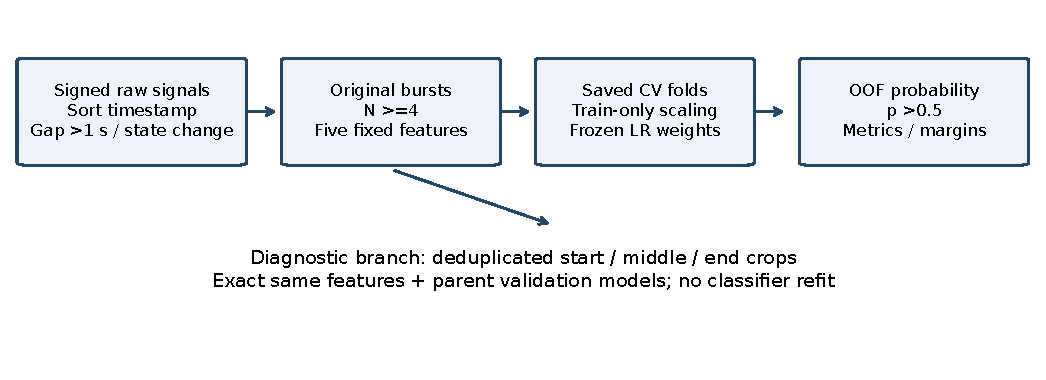
\includegraphics[width=0.96\textwidth]{figures/pipeline.pdf}
\caption{Preserved processing and diagnostic reuse. The existing saved class-weight models are compared on original OOF bursts. Crops use only models for which their parent was a validation burst; classifiers are never refitted on crops.}
\label{fig:pipeline}
\end{figure*}

\subsection{Logistic Regression and Class Weighting}
The saved pipeline fits \texttt{StandardScaler} only on each fold's original training features. For feature $j$, $\tilde{x}_j=(x_j-\mu_{j,\mathrm{train}})/\sigma_{j,\mathrm{train}}$, where the scaler uses population variance. Logistic regression produces
\begin{equation}
z=\boldsymbol{\beta}^{\top}\tilde{\mathbf{x}}+b,
\qquad p=\frac{1}{1+\exp(-z)}.
\end{equation}
The prediction is abnormal exactly when $p>0.5$; equality remains normal, matching the saved binary predictions. Solver \texttt{lbfgs}, $C=1$, maximum iterations 100, tolerance $10^{-4}$, intercept fitting, effective L2 regularization, and recorded random state 42 are preserved. The recorded scikit-learn 1.9.1 parameter representation uses \texttt{penalty='deprecated'} and \texttt{l1\_ratio=0.0}; environment metadata is supplied to avoid silently interpreting this as a different model configuration.

An equivalent weighted L2-penalized objective, up to positive normalization, is
\begin{equation}
\sum_i w_{y_i}\big[-y_i\log p_i-(1-y_i)\log(1-p_i)\big]
+\frac{\|\boldsymbol{\beta}\|_2^2}{2C}.
\end{equation}
We report the existing unweighted condition ($w_0=w_1=1$), manual weights $(1,3)$, $(1,5)$, $(1,10)$, and inverse-frequency balanced weights. Each training fold has 460 normal and 16 abnormal bursts, so balanced weights are $w_0=476/(2\cdot460)=0.517391$ and $w_1=476/(2\cdot16)=14.875$, with ratio 28.75. These absolute weights differ from a manual $(1,28.75)$ pair; at fixed regularization strength, scaling all data-loss weights also changes the loss--penalty balance. The historical artifact additionally contains weights 1:7, 1:15, and 1:20. They are preserved in source copies but are not newly evaluated or used to select the five reported conditions.

\subsection{Validation and Metrics}
The saved \texttt{RepeatedStratifiedKFold} splits use five folds, ten repeats, and random state 42. Every retained burst is a validation burst once per repeat, hence ten OOF appearances. Every validation fold contains 115 normal and four abnormal bursts. The same indices and scaler statistics are reused across class-weight conditions.

Precision is $\mathrm{TP}/(\mathrm{TP}+\mathrm{FP})$, recall is $\mathrm{TP}/(\mathrm{TP}+\mathrm{FN})$, F1 is their harmonic mean, and balanced accuracy averages sensitivity and specificity. We preserve zero-division handling from the saved scoring convention and verify every saved label against $p>0.5$. ROC-AUC uses saved probabilities. PR-AUC is the trapezoidal area returned by integrating precision against recall from \texttt{precision\_recall\_curve}, including its library endpoint convention. Average precision (AP), which uses a different integration rule, is saved separately and never relabeled PR-AUC.

Class-weight summaries are arithmetic means and population standard deviations (ddof 0) over 50 folds, reproducing the existing metric files. These standard deviations describe partition variability, not confidence intervals over independent tests. Repeated folds share bursts and training examples. Crop summaries instead pool positions within each repeat and report means and ddof-0 standard deviations over ten repeats; captions distinguish the two aggregations. The recorded analysis environment is Python 3.11.16, NumPy 2.4.6, pandas 3.0.5, SciPy 1.17.1, and scikit-learn 1.9.1; hardware specifications are not available.

\section{Experiments}
\subsection{Feature Choice and Separability}
The original notebook had already selected the five-feature representation, including removal of AI0 kurtosis using the same evaluation population. We freeze that choice and do not conduct feature selection here. Descriptive separability uses both retained classes, including all 20 abnormal bursts, with feature mean, standard deviation, median, and quartiles. Signed Cohen's $d$ is $(\bar{x}_A-\bar{x}_N)/s_{\mathrm{pooled}}$, using the class-count-weighted pooled sample variance. It is a descriptive standardized difference, not a test of independent acquisition conditions.

For each original validation burst, we recover that fold's scaler from saved original training indices and compute Euclidean distances to the normal and abnormal centroids formed from the training rows only. The normal centroid is the mean of scaled training-normal vectors; the abnormal centroid is defined analogously. Neither validation examples nor crops define these centroids. A saved-coefficient reconstruction reproduces all unweighted original probabilities to maximum absolute error $4.22\times10^{-15}$, without fitting a classifier.

\subsection{Matched Weighting and Persistent Misses}
We pair None and balanced observations by burst identity and original fold. Probability and score changes are $\Delta p=p_{\mathrm{bal}}-p_{\mathrm{None}}$ and $\Delta z=\operatorname{logit}(p_{\mathrm{bal}})-\operatorname{logit}(p_{\mathrm{None}})$. A numerical clipping policy $[10^{-15},1-10^{-15}]$ is declared for logits. No reported probability requires clipping and no selected-weight observation equals zero or one; metrics always use unchanged probabilities.

We count boundary crossings in both directions, separately by class, and report repeated observations and unique parents. For every abnormal burst and weight, saved robustness tables contain TP/FN counts over ten appearances, probability mean/standard deviation/range, and stability. Margin categories are specified before inspecting individual identities: a burst's mean OOF score is positive-margin for $\bar z\geq1$, near-boundary for $|\bar z|<1$, and negative-margin for $\bar z\leq-1$. These are descriptive bins, not tuned decision thresholds; predictions retain the boundary at zero.

\subsection{Frozen-Model Sample-Count Diagnostic}
For targets $L\in\{4,6,8,10,12,15,20,25,30\}$, a parent is eligible when original length $N\geq L$. Crop starts are 0, $\lfloor(N-L)/2\rfloor$, and $N-L$, with identical offsets deduplicated. If $N=L$, precisely one full-parent crop is retained. Each crop recomputes the same signed five features and is scored only in its parent's ten original validation appearances. Classifiers, scalers, features, and threshold are frozen; there is no padding or new training.

Coverage varies with $L$, so each target is paired with full-original predictions from the same eligible parents. A corroborating fixed cohort, $N\geq30$, contains 360 normal and ten abnormal bursts and is held constant across all nine targets. Crop-level metrics treat positions as repeated diagnostic observations. An additional parent-repeat diagnostic averages probabilities across unique positions before applying 0.5; it is saved separately and does not redefine the original protocol.

An original TP parent is affected if any eligible crop/fold becomes FN; persistent crop FN means every crop/fold is FN. Original FNs are included in recall denominators whenever eligible, but excluded from TP-to-FN transition denominators. Feature drift counts each physical crop once, using $|f_{\mathrm{crop}}-f_{\mathrm{parent}}|/s_{f,N}$, where $s_{f,N}$ is the sample standard deviation among the 575 original normal bursts. Raw-unit changes are also saved but cannot fairly rank differently scaled features.

\section{Results}
\subsection{Fixed-Threshold Weighting Trade-Off}
Table~\ref{tab:weights} shows that None and 1:3 tie for the largest reported mean fixed-threshold F1 (0.942), with precision 1.0 and recall 0.9. Balanced weighting reduces precision to 0.725 and F1 to 0.776 without changing recall. Manual weights 1:5 and 1:10 add progressively more false positives. Balanced weighting increases ROC-AUC from 0.917 to 0.948, but trapezoidal PR-AUC decreases from 0.903 to 0.894. Thus the evidence does not establish universal superiority of None: conclusions depend on ranking metric, threshold, and error costs. Figure~\ref{fig:weights} displays the preserved operating-point metrics.

\begin{table*}[t]
\centering
\caption{Class-weight comparison on identical 50 folds, mean $\pm$ population standard deviation (ddof 0). P/R are precision/recall; BA is balanced accuracy. PR-AUC uses trapezoidal integration, not average precision. FP/FN are counts per validation fold.}
\label{tab:weights}
\small
\begin{tabular}{lllllllll}
\toprule
Weight & P & R & F1 & BA & ROC-AUC & PR-AUC & FP/fold & FN/fold \\
\midrule
None & $1.000\pm0.000$ & $0.900\pm0.132$ & $0.942\pm0.079$ & $0.950\pm0.066$ & $0.917\pm0.111$ & $0.903\pm0.128$ & $0.00\pm0.00$ & $0.40\pm0.53$ \\
1:3 & $1.000\pm0.000$ & $0.900\pm0.132$ & $0.942\pm0.079$ & $0.950\pm0.066$ & $0.926\pm0.101$ & $0.904\pm0.127$ & $0.00\pm0.00$ & $0.40\pm0.53$ \\
1:5 & $0.981\pm0.065$ & $0.900\pm0.132$ & $0.931\pm0.080$ & $0.950\pm0.066$ & $0.931\pm0.095$ & $0.904\pm0.127$ & $0.10\pm0.36$ & $0.40\pm0.53$ \\
1:10 & $0.919\pm0.125$ & $0.900\pm0.132$ & $0.898\pm0.094$ & $0.948\pm0.066$ & $0.938\pm0.088$ & $0.903\pm0.126$ & $0.42\pm0.70$ & $0.40\pm0.53$ \\
Balanced & $0.725\pm0.197$ & $0.900\pm0.132$ & $0.776\pm0.113$ & $0.942\pm0.063$ & $0.948\pm0.080$ & $0.894\pm0.122$ & $1.88\pm1.77$ & $0.40\pm0.53$ \\
\bottomrule
\end{tabular}
\end{table*}


\begin{figure}[t]
\centering
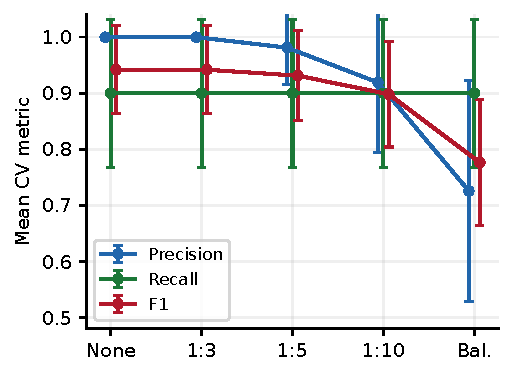
\includegraphics[width=\columnwidth]{figures/class_weight_metrics.pdf}
\caption{Mean fold precision, recall, and F1 with population standard deviations across 50 dependent folds. None and 1:3 share operating-point performance; balanced retains recall while adding false alarms.}
\label{fig:weights}
\end{figure}

Matched analysis finds 94 normal $0\rightarrow1$ prediction crossings, affecting 16 unique normal bursts. No abnormal predictions cross in either direction, and there are no $1\rightarrow0$ crossings in either class. The 94 observations are not 94 independent normal bursts. Both None and balanced detect the same 18 abnormal parents in all ten appearances and miss the same two, bursts 619 and 620, in all ten.

Normal mean OOF probability changes from 0.004682 to 0.096416, with mean score shift $+2.893422$. The 18 detected abnormal bursts have mean probability 0.942362 to 0.963731 and mean score shift $+1.951512$. The two persistent misses have mean probability 0.001180 to 0.036671 and mean shift $+3.110539$, remaining below 0.5 in every appearance. Score shifts are not uniform: 147 normal and 11 detected-abnormal appearances shift negatively. Consequently, this is an observed change in fitted scores, not proof of a pure intercept translation.

\subsection{Most Abnormal Bursts Are Separated; Two Remain Normal-Like}
Figure~\ref{fig:features} shows that the aggregate abnormal feature distribution differs substantially from normal. Signed Cohen's $d$ values are 7.415 for AI0 RMS, 7.785 for AI0 MaxAbs, 2.290 for AI1 RMS, 3.076 for AI1 peak-to-peak, and 1.951 for AI1 kurtosis. These large descriptive differences coexist with persistent individual misses and the acquisition-date confound.

\begin{figure*}[t]
\centering
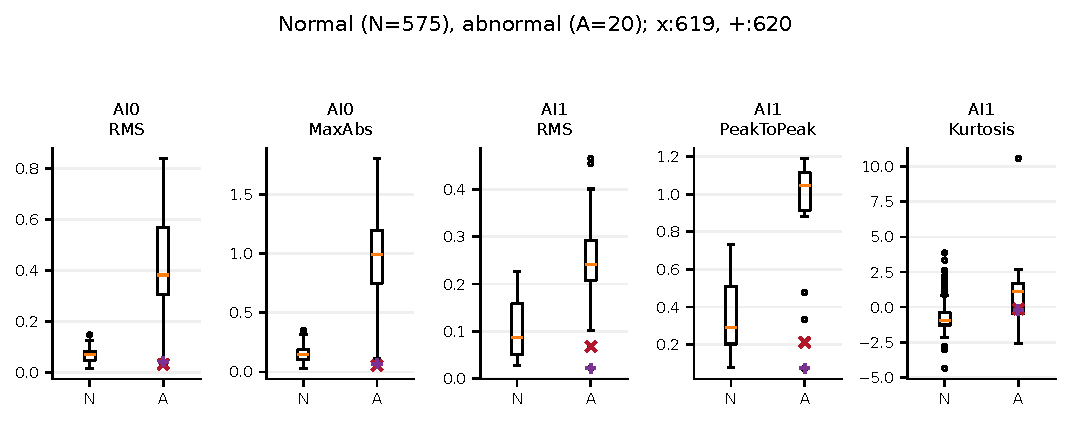
\includegraphics[width=0.96\textwidth]{figures/feature_distributions.pdf}
\caption{Original signed-feature distributions for normal (N=575) and abnormal (A=20) bursts, including both persistent FNs in the abnormal class. Markers identify bursts 619 and 620. Axes retain raw feature units; their scales are not directly comparable.}
\label{fig:features}
\end{figure*}

Under None, mean OOF scores are $-5.720$ for normal, $+3.922$ for all 20 abnormal parents, $+5.122$ for detected abnormal, and $-6.872$ for the two FNs. The score-distribution source table reports mean, median, quartiles, minimum, and maximum for normal and all abnormal, with detected/FN subgroups also retained. All 18 detected abnormal parents have positive-margin mean scores and all two FNs have negative-margin mean scores; none has a near-boundary mean. This parent-mean statement does not require every appearance to have $|z|\geq1$: the lowest detected-abnormal individual score is 0.767. Figure~\ref{fig:probability} separates the missed cases from the detected group.

Table~\ref{tab:fn} reports the two FNs. Their mean distances to the training-normal centroid are 1.271549 and 1.978236, versus 8.627618 and 9.021867 to the training-abnormal centroid. The 18 detected abnormal parents have mean normal-centroid distance 9.515279, with minimum parent-mean distance 5.340304. These geometry and score results support normal-like placement \emph{within this five-feature representation}; they do not establish true signal normality or incorrect labels.

Balanced weighting increases burst 619's mean probability from 0.001333 to 0.021282 and burst 620's from 0.001028 to 0.052060. Their paired mean score shifts are $+2.574060$ and $+3.647018$. Neither is repaired at the retained threshold. This directly tests the persistent-miss part of the hypothesis rather than inferring it from unchanged aggregate recall alone.

\begin{table*}[t]
\centering
\caption{Persistent unweighted false negatives. Distances are means over 10 original OOF appearances to training-only centroids in standardized five-dimensional feature space. Probability standard deviation and per-weight stability are supplied in source tables.}
\label{tab:fn}
\small
\begin{tabular}{rrrrrr}
\toprule
Burst & Length & FN / 10 & Mean $p$ & $d_N$ & $d_A$ \\
\midrule
619 & 10 & 10 & 0.001333 & 1.271549 & 8.627618 \\
620 & 15 & 10 & 0.001028 & 1.978236 & 9.021867 \\
\bottomrule
\end{tabular}
\end{table*}


\begin{figure}[t]
\centering
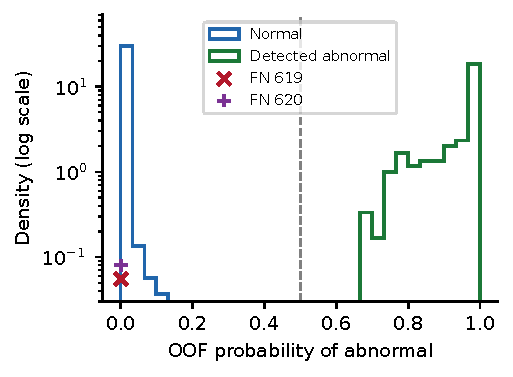
\includegraphics[width=\columnwidth]{figures/none_probability_distribution.pdf}
\caption{Saved unweighted OOF probabilities. Histograms show normal and detected-abnormal densities on a log scale; individual markers show mean probabilities of the two persistent FNs. Histogram observations include dependent repeated appearances.}
\label{fig:probability}
\end{figure}

\subsection{Sample Count and Window Content Affect Frozen Predictions}
Table~\ref{tab:length} distinguishes target-dependent coverage from sample count. At $L=10$, 530 normal and 17 abnormal parents are eligible, with crop recall 0.528571; at $L=15$, 480 normal and 16 abnormal parents are eligible, with recall 0.681818. Original TP parents with at least one crop FN number 12/15 and 9/15 respectively. The $N\geq15$ condition includes the length-15 original TP burst 614; an earlier strictly-shortened $N>15$ analysis had denominator 14, so its 9/14 result is not substituted here. Only burst 603 is FN at every position and fold at these two targets. No normal false positive occurs at any target.

The fixed $N\geq30$ cohort corroborates the trend without changing parent membership: crop recall is 0.820690 at 30 samples, 0.733333 at 25, 0.673333 at 20, 0.600000 at 15, 0.500000 at 12, and 0.496667 at 10, compared with full-original recall 1.0. Among these ten original TP parents, any crop FN affects 8/10 at 15 and 10/10 at 10. The largest adjacent decrease among the listed crop targets is 15 to 12 (ten percentage points in the fixed cohort; 11.93 points in the eligible cohort). This does not identify a unique safe cutoff: cropping at 30 already loses detections, and offsets change alongside duration. Figure~\ref{fig:length} includes same-parent full-original references.

\begin{table*}[t]
\centering
\caption{Frozen unweighted crop inference; eligibility is $N\geq L$. Recall/F1 mean $\pm$ population standard deviation across 10 repeats pooled over crop positions within each repeat, unlike Table~\ref{tab:weights}. Transitions count original-TP parents with any crop/fold FN; the denominator excludes original FNs. Normal FP counts pool repeated crop predictions.}
\label{tab:length}
\small
\begin{tabular}{rlllrlr}
\toprule
$L$ & Normal / abnormal & Recall & F1 & Mean abnormal $p$ & TP $\rightarrow$ FN & Normal FP \\
\midrule
4 & 575/20 & $0.461\pm0.007$ & $0.631\pm0.007$ & 0.4573 & 14/18 & 0 \\
6 & 565/18 & $0.435\pm0.009$ & $0.606\pm0.009$ & 0.4220 & 14/16 & 0 \\
8 & 550/18 & $0.467\pm0.009$ & $0.637\pm0.008$ & 0.4495 & 13/16 & 0 \\
10 & 530/17 & $0.529\pm0.006$ & $0.692\pm0.005$ & 0.5092 & 12/15 & 0 \\
12 & 511/16 & $0.562\pm0.000$ & $0.720\pm0.000$ & 0.5498 & 12/15 & 0 \\
15 & 480/16 & $0.682\pm0.000$ & $0.811\pm0.000$ & 0.6604 & 9/15 & 0 \\
20 & 452/13 & $0.749\pm0.015$ & $0.856\pm0.010$ & 0.7201 & 8/13 & 0 \\
25 & 402/12 & $0.765\pm0.000$ & $0.867\pm0.000$ & 0.7235 & 6/12 & 0 \\
30 & 360/10 & $0.821\pm0.014$ & $0.901\pm0.008$ & 0.7797 & 5/10 & 0 \\
\bottomrule
\end{tabular}
\end{table*}


\begin{figure}[t]
\centering
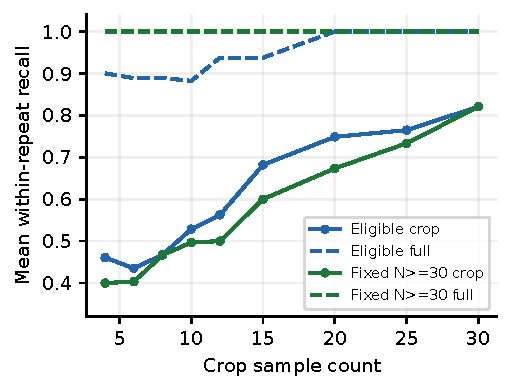
\includegraphics[width=\columnwidth]{figures/sample_count_recall.pdf}
\caption{Frozen unweighted crop recall with full-original predictions of the same eligible parents. The fixed $N\geq30$ cohort controls parent coverage, not crop content. Means pool positions within each repeat.}
\label{fig:length}
\end{figure}

Across the nine targets in the fixed abnormal cohort, the equal-weight mean standardized absolute drift is largest for AI0 RMS (7.802 normal SD), followed by AI0 MaxAbs (7.331), AI1 kurtosis (3.452), AI1 peak-to-peak (2.799), and AI1 RMS (1.356). AI0 MaxAbs is slightly larger than AI0 RMS at 4, 6, 8, and 10 samples; AI0 RMS is larger at the remaining targets. Figure~\ref{fig:drift} therefore supports a duration-dependent sensitivity ranking rather than an invariant single-feature claim.

\begin{figure}[t]
\centering
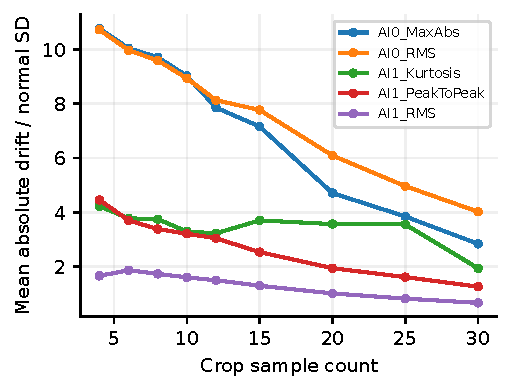
\includegraphics[width=\columnwidth]{figures/sample_count_feature_drift.pdf}
\caption{Absolute feature change per physical crop, divided by the original normal feature SD, for the fixed ten abnormal parents. Repeated model appearances are not counted again.}
\label{fig:drift}
\end{figure}

Burst 619 has ten original samples and 620 has fifteen. Every available crop of both remains FN, and longer targets are explicitly unavailable rather than padded. The broad transition pattern in other original TPs supports a general short-window vulnerability, but cannot identify length alone as the cause of these two original misses. The alternative parent-repeat aggregation also differs from crop-level scoring: fixed-cohort recall is 0.98 at 30, 0.62 at 15, and 0.57 at 10 after averaging position probabilities. These are diagnostic summaries, not replacement official scores.

\section{Discussion}
The data support the hypothesized local mechanism in a restricted sense. Most abnormal bursts are consistently recognized by the existing representation; the remaining two have strongly negative scores and relatively small distances to training-normal feature centroids. Balanced weighting increases their probabilities but does not cross the preserved decision boundary. At the same time, enough normal scores increase to create additional false alarms. Identity-level evidence is essential: equal recall could otherwise conceal a swap between rescued and newly missed examples.

This mechanism does not imply that imbalance has been resolved or that balanced weighting is generally inappropriate. The ROC-AUC improvement shows a ranking benefit despite lower fixed-threshold F1 and PR-AUC. Different false-negative costs, acquisition conditions, representations, or operating thresholds could change the preferred condition. None and 1:3 tie on the reported F1 criterion, so even this dataset does not uniquely select the unweighted setting. No downstream cost model or deployment validation is available.

Class imbalance and minority-sample scarcity are distinct. Loss weighting changes the influence of the observed positives relative to negatives; it does not add independent positive examples, acquisition sessions, or fault mechanisms. The 20 abnormal bursts and their ten repeated validation appearances do not become 200 independent abnormal examples. Even if weighting changed this operating-point result, it would not resolve the limited minority coverage or class--date confound.

The crop analysis also separates representation robustness from label frequency. Global RMS, extrema, and shape estimates change with which samples are retained. A short crop may omit high-amplitude portions or estimate distributional shape from few samples; the present feature drift is compatible with these possibilities but does not isolate a specific physical mechanism. Holding parent membership fixed removes one coverage confound, yet deterministic position and duration remain coupled. We do not infer that longer unavailable versions of bursts 619 or 620 would be detected.

\section{Limitations}
\textbf{Limited and confounded acquisition.} There are only 20 retained abnormal bursts, all from one observed date; normal data occur on a different single date. Session independence and fault diversity are unknown. The classifier may exploit acquisition conditions rather than stable fault signatures. Sensor units, placement, and hardware are unverified.

\textbf{Exploratory selection and evaluation.} The five-feature choice and earlier class-weight comparison use the same observed population. This creates selection optimism; neither nested selection validation nor an external acquisition-day test is supplied. Fifty repeated folds are dependent, and no significance claim is based on treating them as independent experiments. The date confound cannot be resolved by these within-population splits.

\textbf{Representation and protocol constraints.} Summary descriptors discard signal ordering. State-change burst boundaries use labels and require an independent segmentation policy for deployment. Frozen crops alter both available duration and signal content and are dependent descendants of the same parents. They are diagnostics, not new independent validation examples or a causal experiment on original FN length. The fixed threshold is preserved for controlled comparison, not claimed optimal. Centroid proximity is descriptive and does not validate or invalidate labels.

\textbf{Draft status.} This document is an ICML-like two-column article, not an official ICML 2026 template. Citation TODOs, author information, hardware documentation, and independent-data validation must be resolved before submission. The analysis project preserves original inputs and supplies machine checks rather than implying the manuscript is submission-ready.

\section{Conclusion}
For this saved five-feature burst classifier, balanced weighting leaves the same two abnormal bursts missed at threshold 0.5 and adds false-positive decisions among normal bursts. Feature geometry and paired scores support a representation-dependent explanation for this local trade-off. Improved balanced ROC-AUC prevents a broader claim that unweighted training is uniformly better. Frozen-model crops reveal substantial sample-window sensitivity in previously detected abnormal bursts, while leaving the causes of the two original misses unresolved. The next evidential requirement is independent, session-aware acquisition validation with a declared operational cost model; it is not a claim of a new superior detection method.

\section*{References}
\textbf{TODO:} Populate \texttt{references.bib} with author-verified references for the Related Work topics. No fictitious citation is included in this draft.

\end{document}
